\section{Sigma-Delta-DAC}

Die finale Realisierung des DACs erfolgt als \textbf{PWM-DAC}. Die Generierung des PWM-Sigmals erfolgt nach dem Sigma-
Delta-Prinzip

\begin{minipage}[t]{0.58\columnwidth}
    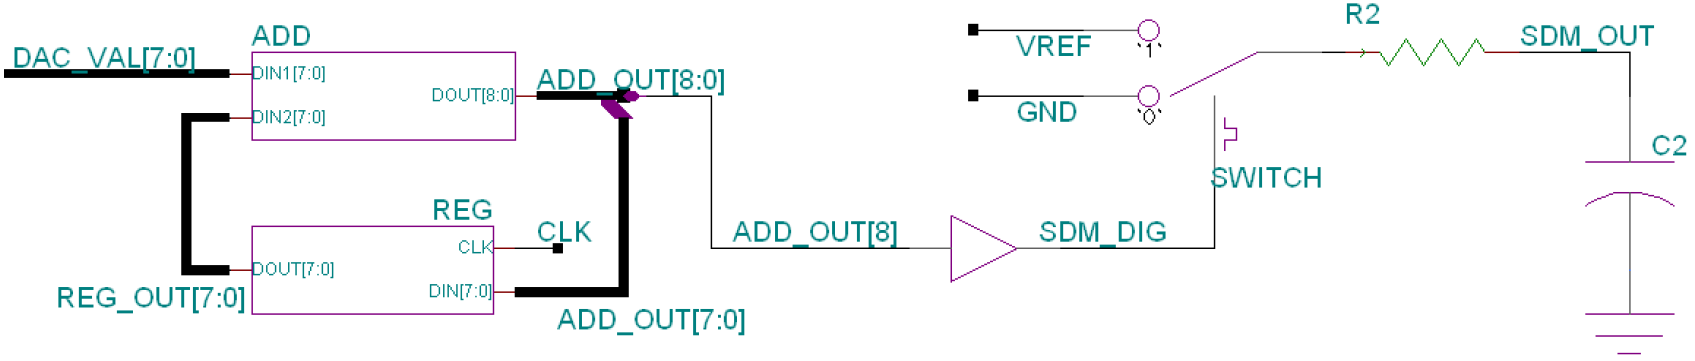
\includegraphics[width=\columnwidth]{images/sigma-delta_DAC.png}
\end{minipage}
\hfill
\begin{minipage}[t]{0.38\columnwidth}
    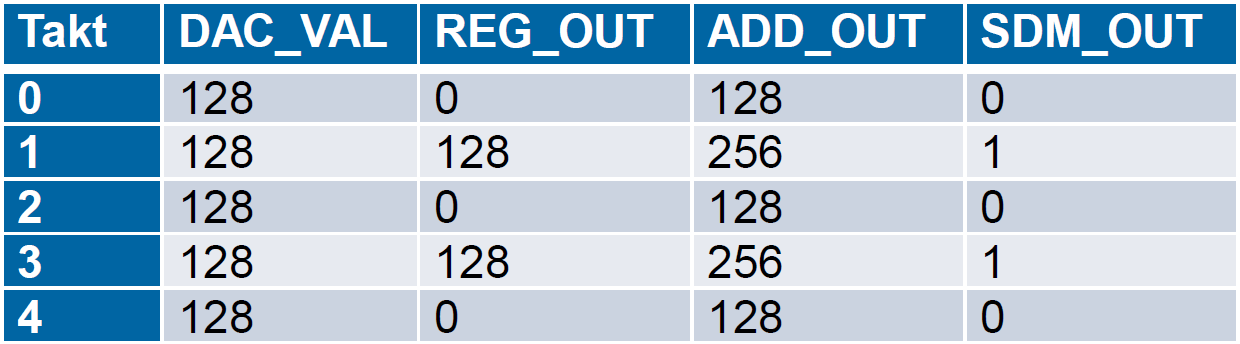
\includegraphics[width=\columnwidth]{images/sigma-delta_DAC_verlauf.png}
\end{minipage}

\subsection{Pattern-Noise}

Für einen 8-Bit DAC ist der digitale Wert $129$ ungünstig, da in der Bitsequenz irgendwann zwei '1' hintereinander auftauchen.
Dies führt zu einer grossen Periodendauer, welche ein \textbf{Pattern Noise} beim DAC verursacht, da die '0' und '1' möglichst
gleichmässig auf die gesamte Periode verteilt werden.


\subsection{Bilanz Sigma-Delta-DAC}

\begin{minipage}[c]{0.48\columnwidth}
    \raggedright%
    \begin{itemize}
        \item Verhalten wie analoger Modulator (Blockschaltbild)
    \end{itemize}

    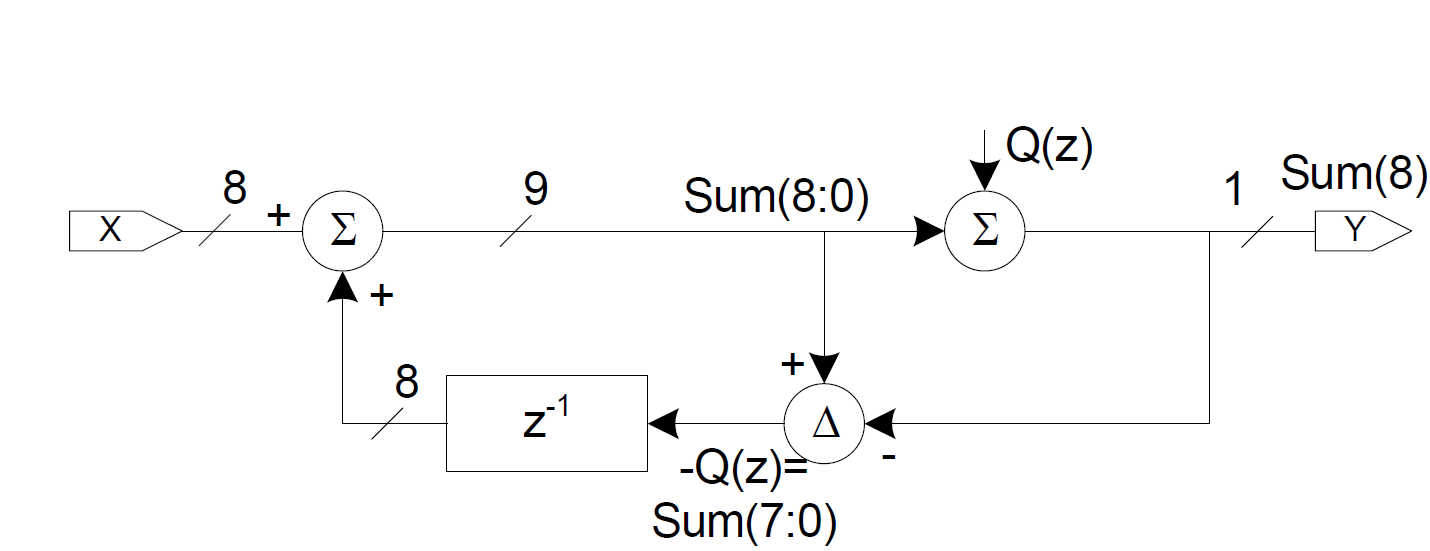
\includegraphics[width=\columnwidth]{images/sigma-delta-DAC_blockschaltbild.png}
\end{minipage}
\hfill
\begin{minipage}[c]{0.48\columnwidth}
    \begin{itemize}
        \item Im Mittel gleich viele '1' und '0' wie bei PWM $= \frac{n}{N}$
        \item '1' werden möglichst gleichmässig in Periode verteilt ($N \cdot T_{\rm clk}$)
        \item Gleichmässige Verteilung ergibt regelmässige Sequenzen \textrightarrow\ periodische Signale \textrightarrow\ unerwünschte
            Frequenzkomponenten (Pattern Noise)
    \end{itemize}
\end{minipage}

